\section{Experiments}

This sections contains experiments regarding the architecture of the variational autoencoder (VAE)
and the quality of the latent space. The experiments use the test and validation data of the RGB
imagery as well as the ground truth semantic labeling and the digital surface models as described in
\autoref{datasets}.

\subsection{Variational Autoencoder Architecture} \label{architecture_experiments}

The experiments presented in this subsection determine the architecture that is used for the further
experiments regarding the latent space in the next subsection. All the tested VAE architectures have 
latent code of the size $1024$ and are trained with $3000$ images over $50$ epochs.
The chosen batch size is $128$ which is base on the results of \textcite{2016-mishkin-systematic} who have analyzed
the impact of multiple learning parameter and architecture choices on the performance of convolutional neural networks.
One conclusion they reach is the suggestion to use batch sizes around 128 or 256.
The training here is done on the personal computer described in \autoref{hardware}.


Regarding the evaluation of the experiments it is interesting how \textcite{2015-theis-generative}
conclude that there are many difficulties in
measuring the optimization and performance of generative models. They find that there is no 
"one-fits-all" metric for the quality of models like variational autoencoders. While the intuitive evaluation
of visual results favors overfitted models, pure reliance on numerical measures is not appropriate when the
goal is image synthesis. Overall the quality of evaluation measure is largely dependent on the application
and goal.
Therefore the performance of the VAEs is on the one hand measured by the mean absolute error (MAE)
between the reconstruction and the input image.
On the other hand it is judged by the subjective opinion of how realistic the reconstructions look and how well
the semantic contents were recreated. This is the case since the MAE 
cannot capture the visual fidelity of a recreation. For instance if a reconstruction was an image that has the mean
color values of the input as every pixel it is just one color in all of the image and only one value was captured
from the input. However, this result has a lower MAE than an image with the inverted values of the
input. Clearly the inverted image is a much better reconstruction of the input than the unicolored image and therefore
additionally judging the results via a visual inspection is necessary.

The VAE architecture descriptions all cover an encoder up to a one dimensional tensor that is fed into two dense
layers which create the means and standard deviations as explained in \autoref{architecture}. Since these two
dense layers, the resampling and the dimension of the latent code is the same for every architecture the following
specifications of encoders do not include these features for brevity.
The inputs for every encoder are $128\times 128$ RGB images, i.e. $128\times 128\times 3$ images. The inputs
for every decoder are the latent code vectors of size $1,024$.


\subsubsection{Number of Convolutions} \label{section_number_of_convolutions_experiment}

This subsection contains 5 tests for which the encoder and decoder architectures are specified in Tables below.
The layers contained by the architecture in a test is specified by the number in the \textit{Test} column as 
described in the tables caption. This means that the test architecture $4$ has $6$ convolutional and
$6$ deconvolutional layers while test $1$ has only $3$ convolutional and $3$ deconvolutional
layers.

\paragraph{Experiment Architectures}

\begin{center}
    \begin{table}[H] 
        \centering
        \begin{tabular}{ | c | l | c | }
            \hline
            Test &Layer & Output\\ \hline
            all &Conv: Kernel $3\times3$, Stride $2\times2$, Filters $8  $    & $64\times 64\times 8  $    \\  
            all &Conv: Kernel $3\times3$, Stride $2\times2$, Filters $16 $    & $32\times 32\times 16 $    \\
            4   &Conv: Kernel $3\times3$, Stride $2\times2$, Filters $32 $    & $16\times 16\times 32 $    \\
            3   &Conv: Kernel $3\times3$, Stride $2\times2$, Filters $64 $    & $8\times 8\times   64 $    \\
            2   &Conv: Kernel $3\times3$, Stride $2\times2$, Filters $128$    & $4\times 4\times   128$    \\
            1   &Conv: Kernel $3\times3$, Stride $2\times2$, Filters $256$    & $2\times 2\times   256$    \\
            all &Flatten                                                              & $1,024$                    \\
            \hline
        \end{tabular} 
        \caption{The layers of the encoder of test $4$ up to the vector that the two dense layers use to produce 
        the means and standard deviations for the latent code. Test $x$ only contains the layers up to
        the layer with $x$ in the \textit{Test} column and the layers with \textit{all}.
        The output of the \textit{Flatten} layer
        varies depending on the test.} \label{table_encoder_num_conv}
    \end{table}
\end{center}
\vspace{-4em}
\begin{center}
    \begin{table}[H]
        \centering
        \begin{tabular}{ | c | l | c | }
            \hline
            Test &Layer & Output\\ \hline
            all &Dense                                                            & $1,024$                   \\
            all &Reshape                                                          & $2\times 2\times    256$  \\
            1   &Deconv: Kernel $3\times3$, Stride $2\times2$, Filters $128$      & $4\times 4\times    128$  \\  
            2   &Deconv: Kernel $3\times3$, Stride $2\times2$, Filters $64 $      & $8\times 8\times    64 $  \\
            3   &Deconv: Kernel $3\times3$, Stride $2\times2$, Filters $32 $      & $16\times 16\times  32 $  \\
            4   &Deconv: Kernel $3\times3$, Stride $2\times2$, Filters $16 $      & $32\times 32\times  16 $  \\
            all &Deconv: Kernel $3\times3$, Stride $2\times2$, Filters $8  $      & $64\times 64\times  8  $  \\
            all &Deconv: Kernel $3\times3$, Stride $2\times2$, Filters $3  $      & $128\times 128\times3  $  \\
            \hline
        \end{tabular} 
        \caption{The layers of the decoder of test $4$. 
        Test $x$ only contains the layers after the layer with the number
        $x$ in the \textit{Test} column and the layers with \textit{all}.
        The outputs of the \textit{Dense} and \textit{Reshape}
        layers vary depending on the test.}
    \end{table}
\end{center}

\pagebreak
\textbf{Results}
\renewcommand{\thesubfigure}{\arabic{subfigure}}
\begin{figure}[H]
    \centering
    \begin{subfigure}{.25\textwidth}
        \centering
        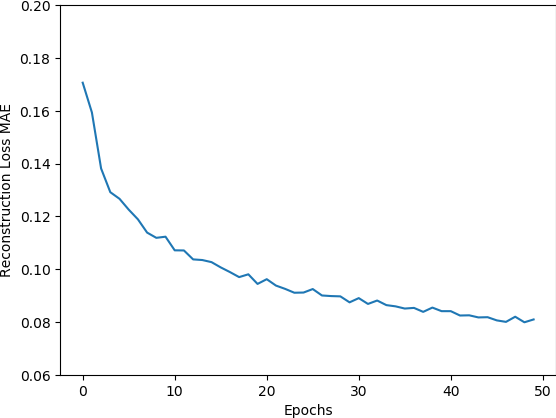
\includegraphics[width=\textwidth]
        {images/figures/experiments_architecture/mae_graphKernel3adjusted2x2x256_dim1024.png}
        \caption{}
    \end{subfigure}%
    \begin{subfigure}{.25\textwidth}
        \centering
        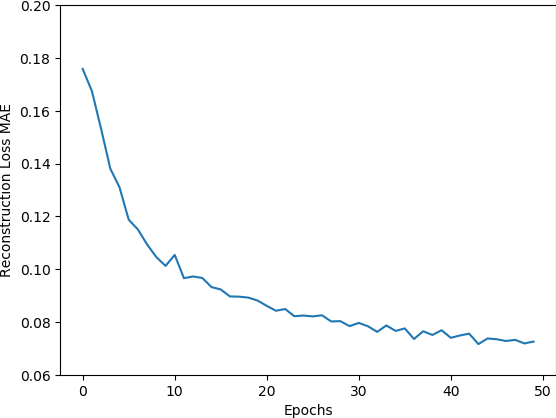
\includegraphics[width=\textwidth]
        {images/figures/experiments_architecture/mae_graphKernel3adjusted4x4x128_dim1024.png}
        \caption{}
    \end{subfigure}%
    \begin{subfigure}{.25\textwidth}
        \centering
        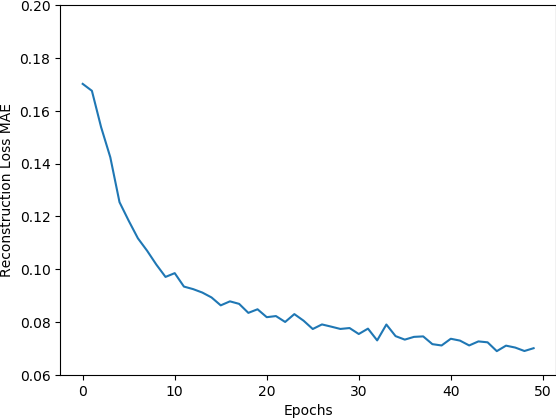
\includegraphics[width=\textwidth]
        {images/figures/experiments_architecture/mae_graphKernel3adjusted8x8x64_dim1024.png}
        \caption{}
    \end{subfigure}%
    \begin{subfigure}{.25\textwidth}
        \centering
        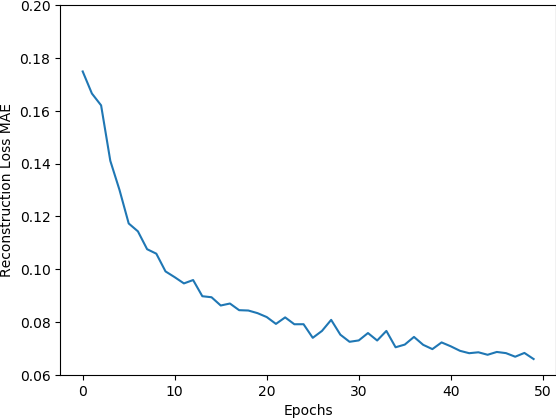
\includegraphics[width=\textwidth]
        {images/figures/experiments_architecture/mae_graphKernel3adjusted16x16x32_dim1024.png}
        \caption{}
    \end{subfigure}
    \caption{There is a graph for each test architecture.
    Each graph depicts the mean MAEs between input and reconstructions across all iterations in an epoch of training.} 
    \label{figure_learning_curves_1}
\end{figure} 

\begin{center}
    \begin{table}[H]
        \centering
        \begin{tabular}{ | c | c | c | c | }
            \hline
            Test &MAEs last Epoch & Loss last Epoch & Training time\\ \hline
            1 & $0.08093627$  & $0.08655346$  & 12 min 58 sec  \\
            2 & $0.07256235$  & $0.07953142$  & 13 min 17 sec  \\
            3 & $0.07004701$  & $0.07820769$  & 14 min 8 sec  \\  
            4 & $0.06594399$  & $0.0751977$  & 15 min 27 sec  \\  
            \hline
        \end{tabular} 
        \caption{For each test architecture the table shows the mean of the MAEs across all iterations of the last
        epoch, the mean loss across all iterations of the last epoch and the time it took to train the model
        on the personal computer as specified in \autoref{hardware}. Note that the loss is not the same
        as MAE since it additionally takes the Kullback-Leibler divergence into account.}  \label{table_mae_1}
    \end{table}
\end{center}

\vspace{-2em}
\begin{figure}[H] 
    \centering
    \begin{subfigure}[t]{.19\textwidth}
        \centering
        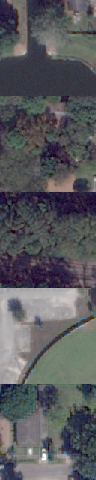
\includegraphics[width=0.5\textwidth]
        {images/figures/experiments_architecture/inputsCol1Kernel3adjusted32x32x32_dim1024.png}\hfill
        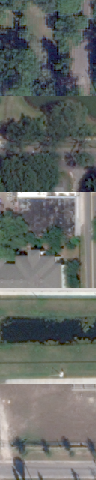
\includegraphics[width=0.5\textwidth]
        {images/figures/experiments_architecture/inputsCol2Kernel3adjusted32x32x32_dim1024.png}
    \end{subfigure}%
    \hspace*{0.1pt}
    \begin{subfigure}[t]{.19\textwidth}
        \centering
        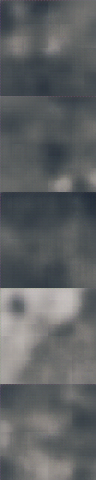
\includegraphics[width=0.5\textwidth]
        {images/figures/experiments_architecture/reconstructionsCol1Kernel3adjusted2x2x256_dim1024.png}\hfill
        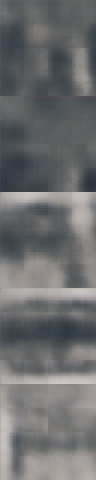
\includegraphics[width=0.5\textwidth]
        {images/figures/experiments_architecture/reconstructionsCol2Kernel3adjusted2x2x256_dim1024.png}
        \caption{}
    \end{subfigure}%
    \hspace*{0.1pt}
    \begin{subfigure}[t]{.19\textwidth}
        \centering
        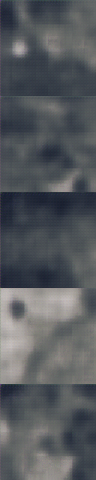
\includegraphics[width=0.5\textwidth]
        {images/figures/experiments_architecture/reconstructionsCol1Kernel3adjusted4x4x128_dim1024.png}\hfill
        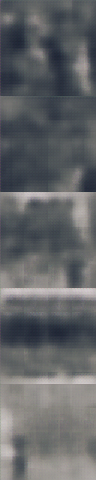
\includegraphics[width=0.5\textwidth]
        {images/figures/experiments_architecture/reconstructionsCol2Kernel3adjusted4x4x128_dim1024.png}
        \caption{}
    \end{subfigure}%
    \hspace*{0.1pt}
    \begin{subfigure}[t]{.19\textwidth}
        \centering
        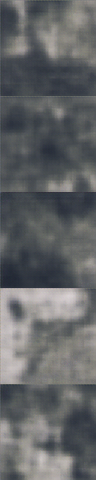
\includegraphics[width=0.5\textwidth]
        {images/figures/experiments_architecture/reconstructionsCol1Kernel3adjusted8x8x64_dim1024.png}\hfill
        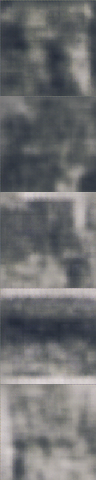
\includegraphics[width=0.5\textwidth]
        {images/figures/experiments_architecture/reconstructionsCol2Kernel3adjusted8x8x64_dim1024.png}
        \caption{}
    \end{subfigure}%
    \hspace*{0.1pt}
    \begin{subfigure}[t]{.19\textwidth}
        \centering
        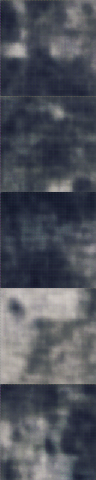
\includegraphics[width=0.5\textwidth]
        {images/figures/experiments_architecture/reconstructionsCol1Kernel3adjusted16x16x32_dim1024.png}\hfill
        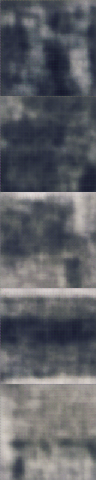
\includegraphics[width=0.5\textwidth]
        {images/figures/experiments_architecture/reconstructionsCol2Kernel3adjusted16x16x32_dim1024.png}
        \caption{}
    \end{subfigure}
    \caption{The left column shows original images taken from a validation set that the VAE has not seen during
    training. The other columns show the reconstructions of the VAE test architectures.} \label{figure_reconstructions_1}
\end{figure} 

\paragraph{Discussion} \mbox{} \\

The learning curves in \autoref{figure_learning_curves_1} show a correlation between the MAE of the
reconstructions and the number of convolutional and deconvolutional layers. The less layers the are the better
the learning curve is which is in line with the visual fidelity of the reconstructions in 
\autoref{figure_reconstructions_1}. The reconstructions of the VAE with the least layers are the sharpest and the 
more layers the VAE has the blurrier the reconstructions are. 

A possible reason for this behavior is that the number of weights in the two dense layers between the 
last convolutional layer and the means and standard deviations increases drastically
if the number of convolutional layers decreases. This is the case because for each additional
value in the last convolutional layer there are $1,024$ additional weights in the three dense layers of the VAE
since $1,024$ is the size of the latent code. For example architecture $1$ only has $3,935,651$ weights while
architecture $2$, with one convolutional and deconvolutional layer less, has $6,492,192$ total weights.
The weights in the dense layers make up most of the total weights
and the higher amount of weights also leads to longer training times as it can be seen in \autoref{table_mae_1}.
However, this increase in training time is negligible compared to the increase of the quality of the reconstructions. 

This leads to the idea that increasing the number of filters, and therefore the size of the dense layers, could yield
better results which is tested in the next section.

\pagebreak
\subsubsection{Number of Filters} \label{section_number_of_filters}

The tables below describe test architectures in a similar way as the previous 
\autoref{section_number_of_convolutions_experiment}. The differences here are that the number of filters is doubled and
the last convolutional layer and the first deconvolutional layer is missing.

\paragraph{Experiment Architectures}

\begin{center}
    \begin{table}[H]
        \centering
        \begin{tabular}{ | c | l | c | }
            \hline
            Test &Layer & Output\\ \hline
            all &Conv: Kernel $3\times3$, Stride $2\times2$, Filters $16 $    & $64\times 64\times 16 $    \\  
            4   &Conv: Kernel $3\times3$, Stride $2\times2$, Filters $32 $    & $32\times 32\times 32 $    \\
            3   &Conv: Kernel $3\times3$, Stride $2\times2$, Filters $64 $    & $16\times 16\times 64 $    \\
            2   &Conv: Kernel $3\times3$, Stride $2\times2$, Filters $128$    & $8\times 8\times   128$    \\
            1   &Conv: Kernel $3\times3$, Stride $2\times2$, Filters $256$    & $4\times 4\times   256$    \\
            all &Flatten                                                      & $2,048$                    \\
            \hline
        \end{tabular} 
        \caption{The layers of the encoder of test $4$ up to the vector that the two dense layers use to produce 
        the means and standard deviations for the latent code. Test $x$ only contains the layers up to
        the layer with $x$ in the \textit{Test} column and the layers with \textit{all}.
         The output of the \textit{Flatten} layer
        varies depending on the test.}
    \end{table}
\end{center}
\vspace{-4em}
\begin{center}
    \begin{table}[H]
        \centering
        \begin{tabular}{ | c | l | c | }
            \hline
            Test &Layer & Output\\ \hline
            all &Dense                                                            & $2,048$                   \\
            all &Reshape                                                          & $4\times 4\times    256$  \\
            1   &Deconv: Kernel $3\times3$, Stride $2\times2$, Filters $128$      & $8\times 8\times    128$  \\
            2   &Deconv: Kernel $3\times3$, Stride $2\times2$, Filters $64 $      & $16\times 16\times  64 $  \\
            3   &Deconv: Kernel $3\times3$, Stride $2\times2$, Filters $32 $      & $32\times 32\times  32 $  \\
            4   &Deconv: Kernel $3\times3$, Stride $2\times2$, Filters $16 $      & $64\times 64\times  16 $  \\
            all &Deconv: Kernel $3\times3$, Stride $2\times2$, Filters $3  $      & $128\times 128\times3  $  \\
            \hline
        \end{tabular}
        \caption{The layers of the decoder of test $4$. 
        Test $x$ only contains the layers after the layer with the number
        $x$ in the \textit{Test} column and the layers with \textit{all}.
        The outputs of the \textit{Dense} and \textit{Reshape}
        layers vary depending on the test.} 
    \end{table}
\end{center}


\pagebreak
\textbf{Results}


\begin{figure}[H]
    \centering
    \begin{subfigure}{.25\textwidth}
        \centering
        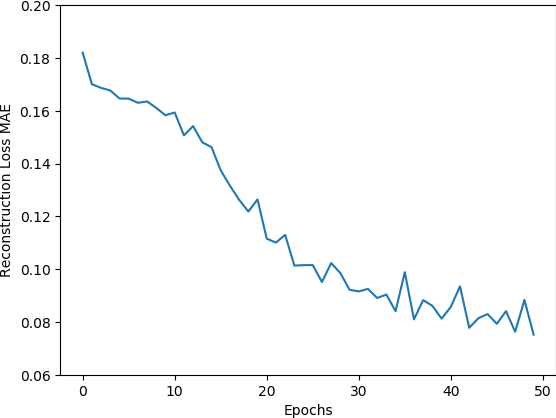
\includegraphics[width=\textwidth]
        {images/figures/experiments_architecture/mae_graphKernel3adjusted4x4x256_dim1024.png}
        \caption{}
    \end{subfigure}%
    \begin{subfigure}{.25\textwidth}
        \centering
        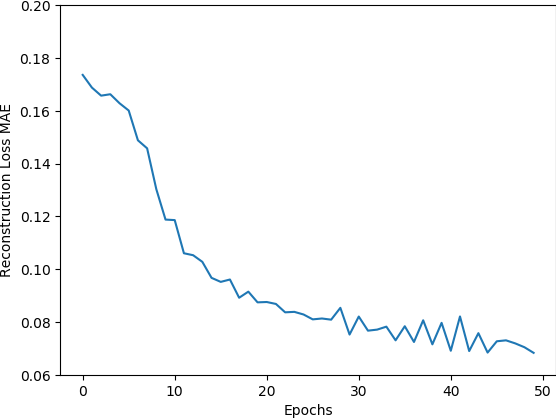
\includegraphics[width=\textwidth]
        {images/figures/experiments_architecture/mae_graphKernel3adjusted8x8x128_dim1024.png}
        \caption{}
    \end{subfigure}%
    \begin{subfigure}{.25\textwidth}
        \centering
        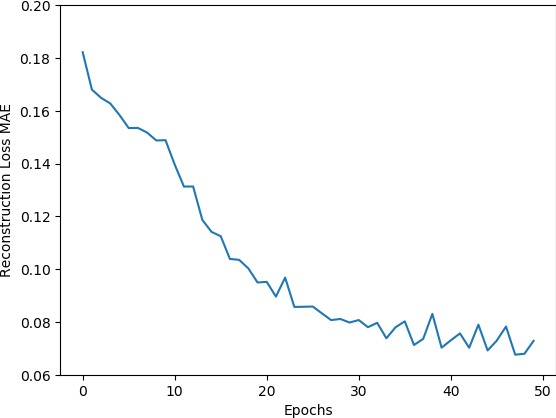
\includegraphics[width=\textwidth]
        {images/figures/experiments_architecture/mae_graphKernel3adjusted16x16x64_dim1024.png}
        \caption{}
    \end{subfigure}%
    \begin{subfigure}{.25\textwidth}
        \centering
        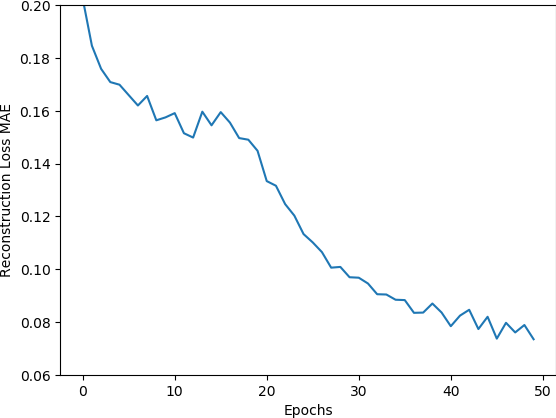
\includegraphics[width=\textwidth]
        {images/figures/experiments_architecture/mae_graphKernel3adjusted32x32x32_dim1024.png}
        \caption{}
    \end{subfigure}
    \caption{There is a graph for each test architecture.
    Each graph depicts the mean MAEs between input and reconstructions 
    across all iterations in an epoch of training.} \label{figure_learning_curves2}
\end{figure} 

\begin{center}
    \begin{table}[H]
        \centering
        \begin{tabular}{ | c | c | c | c | }
            \hline
            Test &MAEs last Epoch & Loss last Epoch & Training time\\ \hline
            1 & $0.07518449$  & $0.08227883$  & 21 min 31 sec  \\
            2 & $0.06828707$  & $0.07637741$  & 22 min 31 sec  \\
            3 & $0.07282908$  & $0.08208682$  & 26 min 17 sec  \\  
            4 & $0.07343805$  & $0.08214357$  & 34 min 31 sec  \\  
            \hline
        \end{tabular} 
        \caption{For each test architecture the table shows the mean of the MAEs across all iterations of the last
        epoch, the mean loss across all iterations of the last epoch and the time it took to train the model
        on the personal computer as described in \autoref{hardware}. Note that the loss is not the same
        as MAE since it additionally takes the Kullback-Leibler divergence into account.} \label{table_maes2}
    \end{table} 
\end{center}


\vspace{-2em}
\begin{figure}[H]
    \centering
    \begin{subfigure}[t]{.19\textwidth}
        \centering
        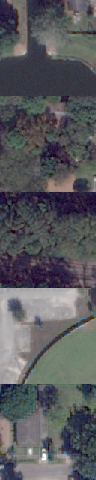
\includegraphics[width=0.5\textwidth]
        {images/figures/experiments_architecture/inputsCol1Kernel3adjusted32x32x32_dim1024.png}\hfill
        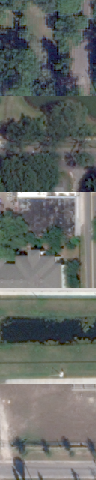
\includegraphics[width=0.5\textwidth]
        {images/figures/experiments_architecture/inputsCol2Kernel3adjusted32x32x32_dim1024.png}
    \end{subfigure}%
    \hspace*{0.1pt}
    \begin{subfigure}[t]{.19\textwidth}
        \centering
        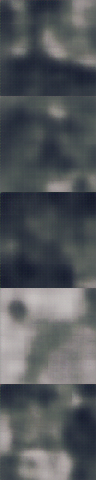
\includegraphics[width=0.5\textwidth]
        {images/figures/experiments_architecture/reconstructionsCol1Kernel3adjusted4x4x256_dim1024.png}\hfill
        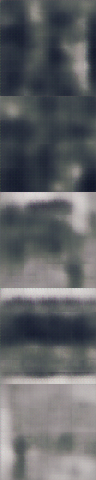
\includegraphics[width=0.5\textwidth]
        {images/figures/experiments_architecture/reconstructionsCol2Kernel3adjusted4x4x256_dim1024.png}
        \caption{}
    \end{subfigure}%
    \hspace*{0.1pt}
    \begin{subfigure}[t]{.19\textwidth}
        \centering
        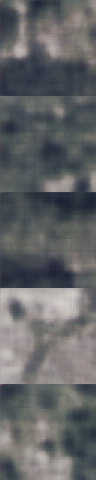
\includegraphics[width=0.5\textwidth]
        {images/figures/experiments_architecture/reconstructionsCol1Kernel3adjusted8x8x128_dim1024.png}\hfill
        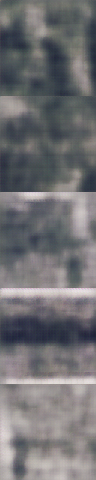
\includegraphics[width=0.5\textwidth]
        {images/figures/experiments_architecture/reconstructionsCol2Kernel3adjusted8x8x128_dim1024.png}
        \caption{}
    \end{subfigure}%
    \hspace*{0.1pt}
    \begin{subfigure}[t]{.19\textwidth}
        \centering
        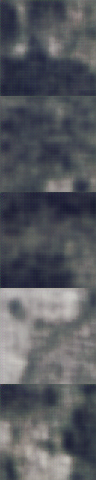
\includegraphics[width=0.5\textwidth]
        {images/figures/experiments_architecture/reconstructionsCol1Kernel3adjusted16x16x64_dim1024.png}\hfill
        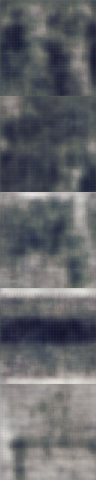
\includegraphics[width=0.5\textwidth]
        {images/figures/experiments_architecture/reconstructionsCol2Kernel3adjusted16x16x64_dim1024.png}
        \caption{}
    \end{subfigure}%
    \hspace*{0.1pt}
    \begin{subfigure}[t]{.19\textwidth}
        \centering
        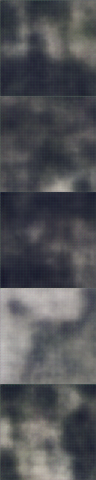
\includegraphics[width=0.5\textwidth]
        {images/figures/experiments_architecture/reconstructionsCol1Kernel3adjusted32x32x32_dim1024.png}\hfill
        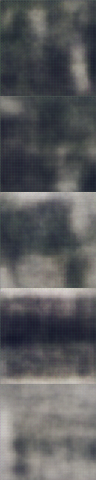
\includegraphics[width=0.5\textwidth]
        {images/figures/experiments_architecture/reconstructionsCol2Kernel3adjusted32x32x32_dim1024.png}
        \caption{}
    \end{subfigure}
    \caption{The left column shows original images taken from a validation set that the VAE has not seen during
    training. The other columns show the reconstructions of the VAE test architectures.}
\end{figure}

\paragraph{Discussion} \mbox{} \\

The trend of less layers correlating with better results does not hold up for the experiments in this subsection when
observing the MAEs in \autoref{table_maes2}. However, the MAEs of the last epoch are not as crucial as in the 
previous subsection since the learning curves in \autoref{figure_learning_curves2} show a lot of variance in 
comparison to the previous subsection. Still the best MAE of the previous architectures beats all results of 
these tests while also taking less than half as long to train and having more realistic looking reconstructions.


\pagebreak
\subsubsection{Kernel Size}

In this subsection the two architectures $4$ and $2$, now called $2$ and $1$,
of the \autoref{section_number_of_convolutions_experiment}
are tested with a kernel size of $5\times 5$ instead of $3\times 3$. These architectures are chosen since architecture
$1$ performed the best so far and a second one is chosen for comparison. 

\paragraph{Results}

\begin{figure}[H]
    \centering
    \begin{subfigure}{.25\textwidth}
        \centering
        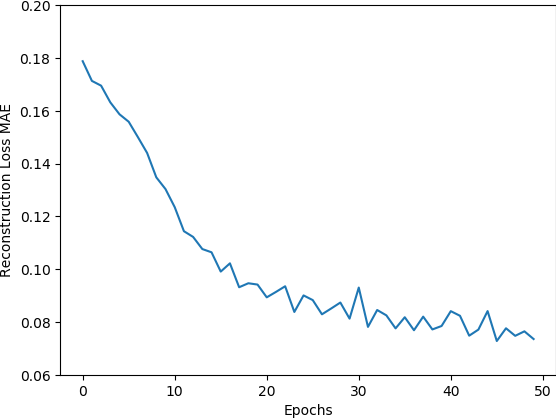
\includegraphics[width=\textwidth]
        {images/figures/experiments_architecture/mae_graphKernel5adjusted16x16x32_dim1024.png}
        \caption{}
    \end{subfigure}%
    \begin{subfigure}{.25\textwidth}
        \centering
        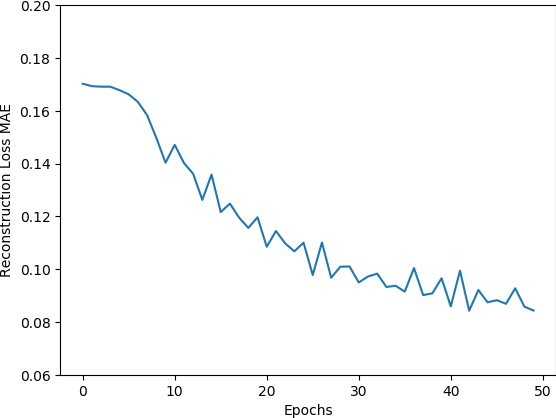
\includegraphics[width=\textwidth]
        {images/figures/experiments_architecture/mae_graphKernel5adjusted4x4x128_dim1024.png}
        \caption{}
    \end{subfigure}
    \caption{There is a graph for each test architecture.
    Each graph depicts the mean MAEs between input and reconstructions across all 
    iterations in an epoch of training.} \label{figure_learning_curves3}
\end{figure} 

\begin{center}
    \begin{table}[H]
        \centering
        \begin{tabular}{ | c | c | c | c | }
            \hline
            Test &MAEs last Epoch & Loss last Epoch & Training time\\ \hline
            1 & $0.08430038$  & $0.08984258$  & 19 min 19 sec  \\  
            2 & $0.07351803$  & $0.08184456$  & 19 min 40 sec  \\  
            \hline
        \end{tabular} 
        \caption{For each test architecture the table shows the mean of the MAEs across all iterations of the last
        epoch, the mean loss across all iterations of the last epoch and the time it took to train the model
        on the personal computer as described in \autoref{hardware}. Note that the loss is not the same
        as MAE since it additionally takes the Kullback-Leibler divergence into account.} \label{table_maes3}
    \end{table} 
\end{center}

\vspace{-2em}
\begin{figure}[H]
    \centering
    \begin{subfigure}[t]{.19\textwidth}
        \centering
        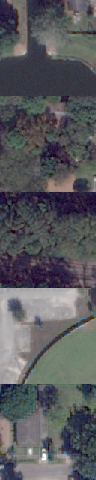
\includegraphics[width=0.5\textwidth]
        {images/figures/experiments_architecture/inputsCol1Kernel3adjusted32x32x32_dim1024.png}\hfill
        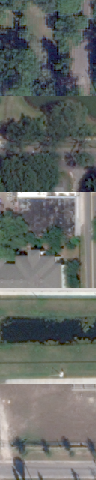
\includegraphics[width=0.5\textwidth]
        {images/figures/experiments_architecture/inputsCol2Kernel3adjusted32x32x32_dim1024.png}
    \end{subfigure}%
    \hspace*{0.1pt}
    \begin{subfigure}[t]{.19\textwidth}
        \centering
        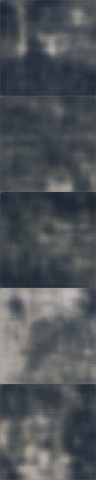
\includegraphics[width=0.5\textwidth]
        {images/figures/experiments_architecture/reconstructionsCol1Kernel5adjusted16x16x32_dim1024.png}\hfill
        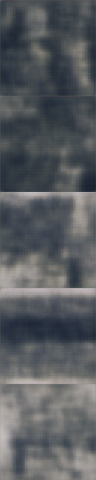
\includegraphics[width=0.5\textwidth]
        {images/figures/experiments_architecture/reconstructionsCol2Kernel5adjusted16x16x32_dim1024.png}
        \caption{}
    \end{subfigure}%
    \hspace*{0.1pt}
    \begin{subfigure}[t]{.19\textwidth}
        \centering
        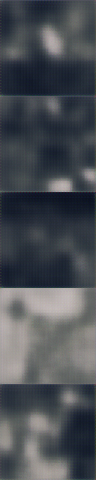
\includegraphics[width=0.5\textwidth]
        {images/figures/experiments_architecture/reconstructionsCol1Kernel5adjusted4x4x128_dim1024.png}\hfill
        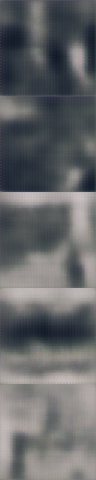
\includegraphics[width=0.5\textwidth]
        {images/figures/experiments_architecture/reconstructionsCol2Kernel5adjusted4x4x128_dim1024.png}
        \caption{}
    \end{subfigure}    
    \caption{The left column shows original images taken from a validation set that the VAE has not seen during
    training. The other columns show the reconstructions of the VAE test architectures.}
\end{figure}

\paragraph{Discussion} \mbox{} \\


The architecture, which had more realistic reconstructions previously, still performs best with the increased
kernel size. However, the reconstructions are all less realistic looking than the ones produced by the 
test architectures with a lower kernel size.

\pagebreak
\subsubsection{Pooling}

This subsection again tests the so far best performing architecture, number $4$ from  
\autoref{section_number_of_convolutions_experiment}, but the convolutional layers now have a stride of $1\times1$
and the dimensionality reduction is done by pooling layers instead as visualized in the tables below. 
Additionally the architecture $3$ from \autoref{section_number_of_filters} is tested 
with similar modifications for comparison. The tests $1$ and $2$ refer to these architectures with max pooling
while $3$ and $4$ refer to the architectures with average pooling.


\paragraph{Experiment Architectures}

\begin{center}
    \begin{table}[H] 
        \centering
        \begin{tabular}{ | l | c | }
            \hline
            Layer & Output\\ \hline
            Conv: Kernel $3\times3$, Stride $1\times1$, Filters $8  $    & $128\times 128\times 8  $    \\
            Pool: Pool size $2\times2$                                   & $64\times 64\times 8  $  \\
            Conv: Kernel $3\times3$, Stride $1\times1$, Filters $16 $    & $64\times 64\times 16 $    \\
            Pool: Pool size $2\times2$                                   & $32\times 32\times 16  $  \\
            Conv: Kernel $3\times3$, Stride $1\times1$, Filters $32 $    & $16\times 16\times 32 $    \\
            Pool: Pool size $2\times2$                                   & $16\times 16\times 32  $  \\
            Flatten                                                              & $1,024$            \\
            \hline
        \end{tabular} 
        \caption{The layers of the encoder of test $1$ up to the vector that the two dense layers use to produce 
        the means and standard deviations for the latent code.} \label{table_encoder_pooling}
    \end{table}
\end{center}
\vspace{-4em}
\begin{center}
    \begin{table}[H]
        \centering
        \begin{tabular}{ | l | c | }
            \hline
            Layer & Output\\ \hline
            Dense                                                            & $1,024$                   \\
            Reshape                                                          & $16\times 16\times  32 $  \\
            Deconv: Kernel $3\times3$, Stride $1\times1$, Filters $16 $      & $32\times 32\times  16 $  \\
            Deconv: Kernel $3\times3$, Stride $1\times1$, Filters $8  $      & $64\times 64\times  8  $  \\
            Deconv: Kernel $3\times3$, Stride $1\times1$, Filters $3  $      & $128\times 128\times3  $  \\
            \hline
        \end{tabular} 
        \caption{The layers of the decoder of test $1$.}
    \end{table}
\end{center}


\pagebreak
\textbf{Results}

\begin{figure}[H]
    \centering
    \begin{subfigure}{.25\textwidth}
        \centering
        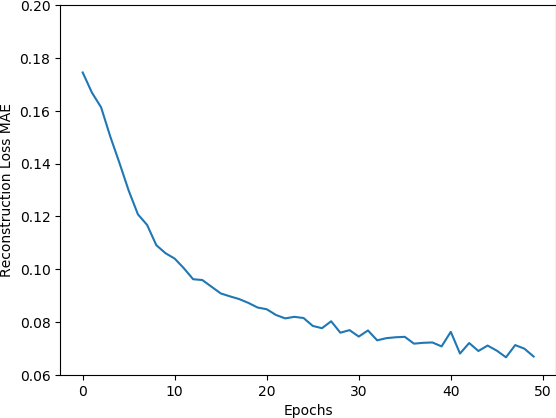
\includegraphics[width=\textwidth]
        {images/figures/experiments_architecture/mae_graphKernel3maxPool16x16x32_dim1024.png}
        \caption{}
    \end{subfigure}%
    \begin{subfigure}{.25\textwidth}
        \centering
        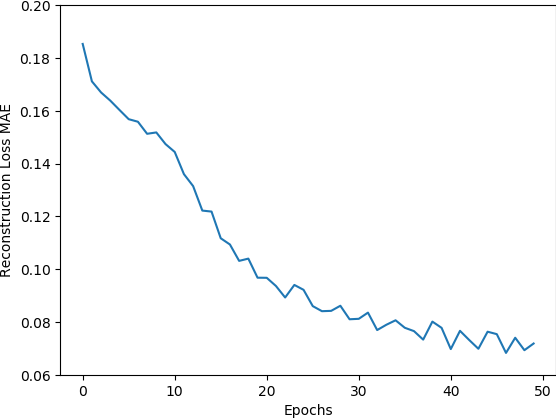
\includegraphics[width=\textwidth]
        {images/figures/experiments_architecture/mae_graphKernel3maxPool16x16x64_dim1024.png}
        \caption{}
    \end{subfigure}%
    \begin{subfigure}{.25\textwidth}
        \centering
        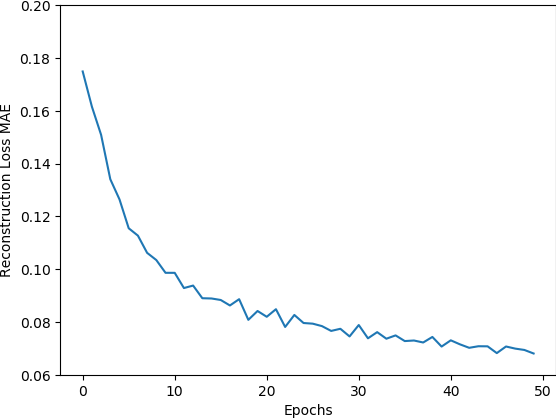
\includegraphics[width=\textwidth]
        {images/figures/experiments_architecture/mae_graphKernel3avgPool16x16x32_dim1024.png}
        \caption{}
    \end{subfigure}%
    \begin{subfigure}{.25\textwidth}
        \centering
        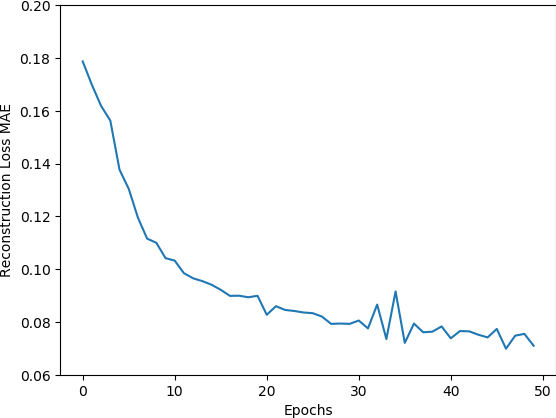
\includegraphics[width=\textwidth]
        {images/figures/experiments_architecture/mae_graphKernel3avgPool16x16x64_dim1024.png}
        \caption{}
    \end{subfigure}
    \caption{There is a graph for each test architecture.
    Each graph depicts the mean MAEs between input and reconstructions across 
    all iterations in an epoch of training.} \label{figure_learning_curves4}
\end{figure} 

\begin{center}
    \begin{table}[H]
        \centering
        \begin{tabular}{ | c | c | c | c | }
            \hline
            Test &MAEs last Epoch & Loss last Epoch & Training time\\ \hline
            1 & $0.07099171$  & $0.07931245$  & 53 min 11 sec  \\
            2 & $0.06803931$  & $0.07641139$  & 30 min 48 sec  \\
            3 & $0.07182192$  & $0.08001233$  & 54 min 9 sec  \\  
            4 & $0.06689975$  & $0.07499783$  & 31 min 39 sec  \\  
            \hline
        \end{tabular} 
        \caption{For each test architecture the table shows the mean of the MAEs across all iterations of the last
        epoch, the mean loss across all iterations of the last epoch and the time it took to train the model
        on the personal computer as described in \autoref{hardware}. Note that the loss is not the same
        as MAE since it additionally takes the Kullback-Leibler divergence into account.} \label{table_maes4}
    \end{table} 
\end{center}

\vspace{-2em}
\begin{figure}[H]
    \centering
    \begin{subfigure}[t]{.19\textwidth}
        \centering
        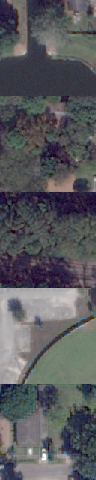
\includegraphics[width=0.5\textwidth]
        {images/figures/experiments_architecture/inputsCol1Kernel3adjusted32x32x32_dim1024.png}\hfill
        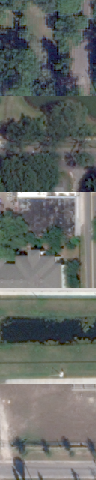
\includegraphics[width=0.5\textwidth]
        {images/figures/experiments_architecture/inputsCol2Kernel3adjusted32x32x32_dim1024.png}
    \end{subfigure}%
    \hspace*{0.1pt}
    \begin{subfigure}[t]{.19\textwidth}
        \centering
        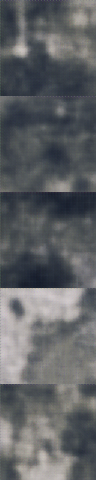
\includegraphics[width=0.5\textwidth]
        {images/figures/experiments_architecture/reconstructionsCol1Kernel3maxPool16x16x32_dim1024.png}\hfill
        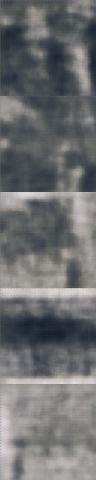
\includegraphics[width=0.5\textwidth]
        {images/figures/experiments_architecture/reconstructionsCol2Kernel3maxPool16x16x32_dim1024.png}
        \caption{}
    \end{subfigure}%
    \hspace*{0.1pt}
    \begin{subfigure}[t]{.19\textwidth}
        \centering
        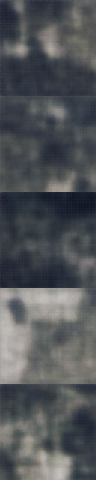
\includegraphics[width=0.5\textwidth]
        {images/figures/experiments_architecture/reconstructionsCol1Kernel3maxPool16x16x64_dim1024.png}\hfill
        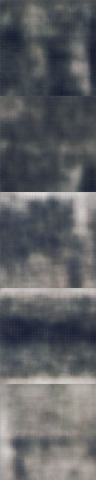
\includegraphics[width=0.5\textwidth]
        {images/figures/experiments_architecture/reconstructionsCol2Kernel3maxPool16x16x64_dim1024.png}
        \caption{}
    \end{subfigure}%
    \hspace*{0.1pt}
    \begin{subfigure}[t]{.19\textwidth}
        \centering
        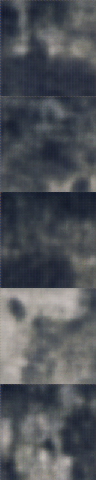
\includegraphics[width=0.5\textwidth]
        {images/figures/experiments_architecture/reconstructionsCol1Kernel3avgPool16x16x32_dim1024.png}\hfill
        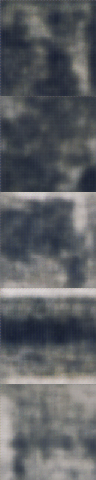
\includegraphics[width=0.5\textwidth]
        {images/figures/experiments_architecture/reconstructionsCol2Kernel3avgPool16x16x32_dim1024.png}
        \caption{}
    \end{subfigure}%
    \hspace*{0.1pt}
    \begin{subfigure}[t]{.19\textwidth}
        \centering
        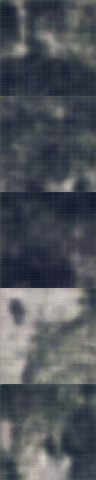
\includegraphics[width=0.5\textwidth]
        {images/figures/experiments_architecture/reconstructionsCol1Kernel3avgPool16x16x64_dim1024.png}\hfill
        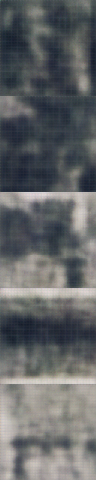
\includegraphics[width=0.5\textwidth]
        {images/figures/experiments_architecture/reconstructionsCol2Kernel3avgPool16x16x64_dim1024.png}
        \caption{}
    \end{subfigure}
    \caption{The left column shows original images taken from a validation set that the VAE has not seen during
    training. The other columns show the reconstructions of the VAE test architectures.}
\end{figure}

\paragraph{Discussion} \mbox{} \\


Regarding the results in Table \autoref{table_maes4} it could be argued that pooling just led to worse results with
MAEs that are a bit worse and training times that are far longer. However, the visual fidelity of the recreations
is judged as the best for architecture $4$ of this subsection.


\subsubsection{Best Architectures}

The two architectures that came out as the best regarding visual fidelity and the MAE between inputs and 
reconstructions are number $4$ from \autoref{section_number_of_convolutions_experiment} and the architecture
with max pooling. These are also the architectures presented in \autoref{architecture} that are used
for the further experiments regarding the latent space. The following \autoref{figure_results_trained_on_all}
shows the reconstructions of these architectures trained on the full training set of $178,112$ images instead
of just $3000$ images. The size of the latent code is $1,024$ again.

As expected the reconstructions are a lot better and apart from a bit of blur they look the same as the originals
while the pooling architecture creates more blur than the fully convolutional architecture.

\renewcommand{\thesubfigure}{\alph{subfigure}}
\begin{figure}[H]
    \centering
    \begin{subfigure}[t]{.19\textwidth}
        \centering
        \includegraphics[width=0.5\textwidth]
        {images/figures/experiments_architecture/inputsCol1Kernel3adjusted32x32x32_dim1024.png}\hfill
        \includegraphics[width=0.5\textwidth]
        {images/figures/experiments_architecture/inputsCol2Kernel3adjusted32x32x32_dim1024.png}
    \end{subfigure}%
    \hspace*{0.1pt}
    \begin{subfigure}[t]{.19\textwidth}
        \centering
        \includegraphics[width=0.5\textwidth]
        {images/figures/experiments_architecture/reconstructionsCol116x16x32TRAINEDON178000_dim1024.png}\hfill
        \includegraphics[width=0.5\textwidth]
        {images/figures/experiments_architecture/reconstructionsCol216x16x32TRAINEDON178000_dim1024.png}
        \caption{}
    \end{subfigure}%
    \hspace*{0.1pt}
    \begin{subfigure}[t]{.19\textwidth}
        \centering
        \includegraphics[width=0.5\textwidth]
        {images/figures/experiments_architecture/reconstructionsCol116x16x32maxPoolTRAINEDON178000_dim1024.png}\hfill
        \includegraphics[width=0.5\textwidth]
        {images/figures/experiments_architecture/reconstructionsCol216x16x32maxPoolTRAINEDON178000_dim1024.png}
        \caption{}
    \end{subfigure}
    \caption{The left column shows original images taken from a validation set that the VAE has not seen during
    training. Column $(a)$ shows the reconstructions of the fully convolutional VAE while column $(b)$ 
    depicts the reconstructions of the max pooling architecture.} \label{figure_results_trained_on_all}
\end{figure} 
 

\subsection{Latent Space} \label{latent_space_experiments}

The results below visualize two dimensional data points that represent a latent code which then again corresponds
to an input image. The dimensionality reduction from the high dimensional latent space to two dimensional space
is done via t-SNE as  explained in \autoref{section_understanding_latent_space}.

After PCA and t-SNE is used to reduce the dimensions of the latent code to 2, the low dimensional representation can be
plotted in a scatter plot. This way it becomes evident if the autoencoder has learned any distinct clusters.
To recap, every point in those plots is a low dimensional representation of a latent code that corresponds to
a $128 \times 128$ section of an RGB satellite image. 
Now the goal is to find out what features the learned clusters in the plots correspond to. For that purpose the
semantic labeling and digital surface models, \autoref{datasets}, are used. In the first type of plot the points
are colored according to the most dominant class in the corresponding image. Those classes are building, vegetation,
water, ground and clutter. In the second kind of plot the points have a gray value equal to the average pixel
values in the digital surface models meaning that points for images that have on average more heights are brighter
than points representing images with less heights.
In a third type of plot the points are represented by the corresponding images themselves.
In those plots it can be observed if the clusters correlate to one of the visualized features which would mean that
the autoencoder has learned to cluster that feature.

All the plots in the following subsections display points for $4000$ images.

\subsubsection{Fully convolutional Architecture}
When observing the following two figures it first of all becomes evident that the VAEs have generated some clusters
which is more clear in the visualizations produced with t-SNE than in those produced with PCA.

Regarding the question of what features the learned clusters correspond to, the plots colored by dominant class
reveal that the VAEs have learned to distinguish water (colored blue) and vegetation (colored green) from the rest 
to a reasonable degree. Especially the t-SNE visualization for coding size $50$ shows a very distinct cluster
with all water images and two close clusters for most of the vegetation images.
However, the same can not be said for height information. The overall high and low images are almost all 
evenly distributed across all clusters with only a single cluster appearing slightly darker, i.e. higher, than the
rest. This suggests the VAEs have learned the topographic classes vegetation and water as features while not 
distinguishing by height up to the latent layer. 


\begin{figure}[H]
    \centering
    \begin{subfigure}{.25\textwidth}
        \centering
        \includegraphics[width=\textwidth]{images/figures/experiments_latent/convolutional_dim1024_PCA_classes.png}
    \end{subfigure}%
    \begin{subfigure}{.25\textwidth}
        \centering
        \includegraphics[width=\textwidth]{images/figures/experiments_latent/convolutional_dim512_PCA_classes.png}
    \end{subfigure}%
    \begin{subfigure}{.25\textwidth}
        \centering
        \includegraphics[width=\textwidth]{images/figures/experiments_latent/convolutional_dim128_PCA_classes.png}
    \end{subfigure}%
    \begin{subfigure}{.25\textwidth}
        \centering
        \includegraphics[width=\textwidth]{images/figures/experiments_latent/convolutional_dim50_PCA_classes.png}
    \end{subfigure}
    \begin{subfigure}{.25\textwidth}
        \centering
        \includegraphics[width=\textwidth]{images/figures/experiments_latent/convolutional_dim1024_classes.png}
        \caption{Code size: $1,024$}
    \end{subfigure}%
    \begin{subfigure}{.25\textwidth}
        \centering
        \includegraphics[width=\textwidth]{images/figures/experiments_latent/convolutional_dim512_classes.png}
        \caption{Code size: $512$}
    \end{subfigure}%
    \begin{subfigure}{.25\textwidth}
        \centering
        \includegraphics[width=\textwidth]{images/figures/experiments_latent/convolutional_dim128_classes.png}   
        \caption{Code size: $128$}
    \end{subfigure}%
    \begin{subfigure}{.25\textwidth}
        \centering
        \includegraphics[width=\textwidth]{images/figures/experiments_latent/convolutional_dim50_classes.png}
        \caption{Code size: $50$}
    \end{subfigure}
    \caption{PCA results in the top row. 
    T-SNE results in the bottom row. 
    The coloring corresponds to the predominant classes in the input images with green for vegetation, 
    grey for ground, blue for water, red for buildings and yellow for clutter.} \label{figure_classes_convolutional}
\end{figure} 

\begin{figure}[H]
    \centering
    \begin{subfigure}{.25\textwidth}
        \centering
        \includegraphics[width=\textwidth]{images/figures/experiments_latent/convolutional_dim1024_PCA_dsm.png}
    \end{subfigure}%
    \begin{subfigure}{.25\textwidth}
        \centering
        \includegraphics[width=\textwidth]{images/figures/experiments_latent/convolutional_dim512_PCA_dsm.png}
    \end{subfigure}%
    \begin{subfigure}{.25\textwidth}
        \centering
        \includegraphics[width=\textwidth]{images/figures/experiments_latent/convolutional_dim128_PCA_dsm.png}
    \end{subfigure}%
    \begin{subfigure}{.25\textwidth}
        \centering
        \includegraphics[width=\textwidth]{images/figures/experiments_latent/convolutional_dim50_PCA_dsm.png}
    \end{subfigure}
    \begin{subfigure}{.25\textwidth}
        \centering
        \includegraphics[width=\textwidth]{images/figures/experiments_latent/convolutional_dim1024_dsm.png}
        \caption{Code size: $1,024$}
    \end{subfigure}%
    \begin{subfigure}{.25\textwidth}
        \centering
        \includegraphics[width=\textwidth]{images/figures/experiments_latent/convolutional_dim512_dsm.png}
        \caption{Code size: $512$}
    \end{subfigure}%
    \begin{subfigure}{.25\textwidth}
        \centering
        \includegraphics[width=\textwidth]{images/figures/experiments_latent/convolutional_dim128_dsm.png}  
        \caption{Code size: $128$} 
    \end{subfigure}%
    \begin{subfigure}{.25\textwidth}
        \centering
        \includegraphics[width=\textwidth]{images/figures/experiments_latent/convolutional_dim50_dsm.png}
        \caption{Code size: $50$}
    \end{subfigure}
    \caption{PCA results in the top row. 
    T-SNE results in the bottom row.  
    The coloring corresponds to the average of the height values in the digital surface model for the
    input image. Darker points represent a higher average height.} \label{figure_heights_convolutional}
\end{figure}

The figure below only features the results of t-SNE since the PCA visualizations offer no additional insights.
The most obvious of those insights is that the learned clusters correspond to the average color of the images.
While this is rather easy to learn a closer inspection of the clusters show that the VAE has also learned far
more complicated features which can be seen in \autoref{figure_closer_clusters}. The VAEs also seem to
cluster by the direction of edges and higher level features like types of roads with images of different sections
of the same road always being in the same cluster.\\

The t-SNE visualizations also show much more distinct clusters for different high level features if the coding
size is lower with the coding size $50$ yielding the most obvious clusters. This suggests that the smaller
latent space forces the VAE to learn and cluster high level features in an increased fashion. However, 
the reason for the better clustering might also simply be that the smaller latent representations are easier
to interpret and therefore the t-SNE algorithm is abled to retain more of the structure in the high dimensional
space.
If the improved visualization is the result of the learning behavior of the VAE 
it means that there is a tradeoff between a more interpretable latent space with 
good clustering and the reconstruction quality. This is the case because a smaller latent dimension 
means worse reconstructions
since the VAE has to fit the same information into a smaller vector. This can also be seen in
\autoref{figure_reconstructions_convolutional}.

\begin{figure}[H]
    \centering
    \begin{subfigure}{.5\textwidth}
        \centering
        \includegraphics[width=\textwidth]{images/figures/experiments_latent/convolutional_dim1024_images.png}
        \caption{Code size: $1,024$}
    \end{subfigure}%
    \begin{subfigure}{.5\textwidth}
        \centering
        \includegraphics[width=\textwidth]{images/figures/experiments_latent/convolutional_dim512_images.png}
        \caption{Code size: $512$}
    \end{subfigure}
    \begin{subfigure}{.5\textwidth}
        \centering
        \includegraphics[width=\textwidth]{images/figures/experiments_latent/convolutional_dim128_images.png}   
        \caption{Code size: $128$}
    \end{subfigure}%
    \begin{subfigure}{.5\textwidth}
        \centering
        \includegraphics[width=\textwidth]{images/figures/experiments_latent/convolutional_dim50_images.png}
        \caption{Code size: $50$}
    \end{subfigure}
    \caption{Two dimensional output points of t-SNE of $4000$ latent codes. The points are represented by the input
    images that produced the latent code corresponding 
    to the two dimensional representation.} \label{figure_images_convolutional_tsne}
\end{figure} 

\begin{figure}[H]
    \centering
    \begin{subfigure}[t]{.19\textwidth}
        \centering
        \includegraphics[width=0.5\textwidth]
        {images/figures/experiments_architecture/inputsCol1Kernel3adjusted32x32x32_dim1024.png}\hfill
        \includegraphics[width=0.5\textwidth]
        {images/figures/experiments_architecture/inputsCol2Kernel3adjusted32x32x32_dim1024.png}
    \end{subfigure}%
    \hspace*{0.1pt}
    \begin{subfigure}[t]{.19\textwidth}
        \centering
        \includegraphics[width=0.5\textwidth]
        {images/figures/experiments_architecture/reconstructionsCol116x16x32TRAINEDON178000_dim1024.png}\hfill
        \includegraphics[width=0.5\textwidth]
        {images/figures/experiments_architecture/reconstructionsCol216x16x32TRAINEDON178000_dim1024.png}
        \caption{$1024$}
    \end{subfigure}%
    \hspace*{0.1pt}
    \begin{subfigure}[t]{.19\textwidth}
        \centering
        \includegraphics[width=0.5\textwidth]
        {images/figures/experiments_latent/reconstructionsCol116x16x32TRAINEDON178000_dim512.png}\hfill
        \includegraphics[width=0.5\textwidth]
        {images/figures/experiments_latent/reconstructionsCol216x16x32TRAINEDON178000_dim512.png}
        \caption{$512$}
    \end{subfigure}%
    \hspace*{0.1pt}
    \begin{subfigure}[t]{.19\textwidth}
        \centering
        \includegraphics[width=0.5\textwidth]
        {images/figures/experiments_latent/reconstructionsCol116x16x32TRAINEDON178000_dim128.png}\hfill
        \includegraphics[width=0.5\textwidth]
        {images/figures/experiments_latent/reconstructionsCol216x16x32TRAINEDON178000_dim128.png}
        \caption{$128$}
    \end{subfigure}%
    \hspace*{0.1pt}
    \begin{subfigure}[t]{.19\textwidth}
        \centering
        \includegraphics[width=0.5\textwidth]
        {images/figures/experiments_latent/reconstructionsCol116x16x32TRAINEDON178000_dim50.png}\hfill
        \includegraphics[width=0.5\textwidth]
        {images/figures/experiments_latent/reconstructionsCol216x16x32TRAINEDON178000_dim50.png}
        \caption{$50$}
    \end{subfigure}
    \caption{The left column shows original images taken from a validation set that the VAE has not seen during
    training. The other columns show the reconstructions produced by the VAEs with the different coding sizes.}
    \label{figure_reconstructions_convolutional}
\end{figure} 


\begin{figure}[H]
    \centering
    \begin{subfigure}{.5\textwidth}
        \centering
        \includegraphics[width=\textwidth]
        {images/figures/experiments_latent/convolutional_dim50_images_sideways_street.png}
    \end{subfigure}%
    \begin{subfigure}{.5\textwidth}
        \centering
        \includegraphics[width=\textwidth]
        {images/figures/experiments_latent/convolutional_dim50_images_sideways_street3.png}
    \end{subfigure}
    \begin{subfigure}{.5\textwidth}
        \centering
        \includegraphics[width=\textwidth]
        {images/figures/experiments_latent/convolutional_dim50_images_upwards_observation.png}  
    \end{subfigure}%
    \begin{subfigure}{.5\textwidth}
        \centering
        \includegraphics[width=\textwidth]
        {images/figures/experiments_latent/convolutional_dim50_images_sideways_other_street.png}
    \end{subfigure}
    \caption{Clusters of VAE with coding size $50$}
    \label{figure_closer_clusters}
\end{figure} 





\subsubsection{Pooling Architecture}

The hypothesis is that the invariances introduced by the pooling layers force the VAE to learn more higher level
features than the fully convolutional architecture. However, this does not seem to be the case since the 
figures below show almost exactly the same results as the fully convolutional
VAE in the previous subsection. This means that the tested pooling architecture offers no advantages with the
quality of the latent space being equal while producing worse reconstructions as it was seen in 
\autoref{architecture_experiments}. The convolutional VAE seems to implicitly learn the invariances introduced by
the pooling layers.

\begin{figure}[H]
    \centering
    \begin{subfigure}{.25\textwidth}
        \centering
        \includegraphics[width=\textwidth]{images/figures/experiments_latent/pooling_dim1024_PCA_classes.png}
    \end{subfigure}%
    \begin{subfigure}{.25\textwidth}
        \centering
        \includegraphics[width=\textwidth]{images/figures/experiments_latent/pooling_dim512_PCA_classes.png}
    \end{subfigure}%
    \begin{subfigure}{.25\textwidth}
        \centering
        \includegraphics[width=\textwidth]{images/figures/experiments_latent/pooling_dim128_PCA_classes.png}
    \end{subfigure}%
    \begin{subfigure}{.25\textwidth}
        \centering
        \includegraphics[width=\textwidth]{images/figures/experiments_latent/pooling_dim50_PCA_classes.png}
    \end{subfigure}
    \begin{subfigure}{.25\textwidth}
        \centering
        \includegraphics[width=\textwidth]{images/figures/experiments_latent/pooling_dim1024_classes.png}
        \caption{Code size: $1,024$}
    \end{subfigure}%
    \begin{subfigure}{.25\textwidth}
        \centering
        \includegraphics[width=\textwidth]{images/figures/experiments_latent/pooling_dim512_classes.png}
        \caption{Code size: $512$}
    \end{subfigure}%
    \begin{subfigure}{.25\textwidth}
        \centering
        \includegraphics[width=\textwidth]{images/figures/experiments_latent/pooling_dim128_classes.png}   
        \caption{Code size: $128$}
    \end{subfigure}%
    \begin{subfigure}{.25\textwidth}
        \centering
        \includegraphics[width=\textwidth]{images/figures/experiments_latent/pooling_dim50_classes.png}
        \caption{Code size: $50$}
    \end{subfigure}
    \caption{ PCA results in the top row. 
    T-SNE results in the bottom row. 
    The coloring represents the predominant class in the input with green for vegetation, 
    grey for ground, blue for water, red for buildings and yellow for clutter.} \label{figure_classes_pooling}
\end{figure} 

\begin{figure}[H]
    \centering
    \begin{subfigure}{.25\textwidth}
        \centering
        \includegraphics[width=\textwidth]{images/figures/experiments_latent/pooling_dim1024_PCA_dsm.png}
    \end{subfigure}%
    \begin{subfigure}{.25\textwidth}
        \centering
        \includegraphics[width=\textwidth]{images/figures/experiments_latent/pooling_dim512_PCA_dsm.png}
    \end{subfigure}%
    \begin{subfigure}{.25\textwidth}
        \centering
        \includegraphics[width=\textwidth]{images/figures/experiments_latent/pooling_dim128_PCA_dsm.png}
    \end{subfigure}%
    \begin{subfigure}{.25\textwidth}
        \centering
        \includegraphics[width=\textwidth]{images/figures/experiments_latent/pooling_dim50_PCA_dsm.png}
    \end{subfigure}
    \begin{subfigure}{.25\textwidth}
        \centering
        \includegraphics[width=\textwidth]{images/figures/experiments_latent/pooling_dim1024_dsm.png}
        \caption{Code size: $1,024$}
    \end{subfigure}%
    \begin{subfigure}{.25\textwidth}
        \centering
        \includegraphics[width=\textwidth]{images/figures/experiments_latent/pooling_dim512_dsm.png}
        \caption{Code size: $512$}
    \end{subfigure}%
    \begin{subfigure}{.25\textwidth}
        \centering
        \includegraphics[width=\textwidth]{images/figures/experiments_latent/pooling_dim128_dsm.png}  
        \caption{Code size: $128$} 
    \end{subfigure}%
    \begin{subfigure}{.25\textwidth}
        \centering
        \includegraphics[width=\textwidth]{images/figures/experiments_latent/pooling_dim50_dsm.png}
        \caption{Code size: $50$}
    \end{subfigure}
    \caption{PCA results in the top row. 
    T-SNE results in the bottom row. 
    The coloring corresponds to the average of the height values in the digital surface model for the
    input image. Darker points represent a higher average height.} \label{figure_heights_pooling}
\end{figure}


\begin{figure}[H]
    \centering
    \begin{subfigure}{.5\textwidth}
        \centering
        \includegraphics[width=\textwidth]{images/figures/experiments_latent/pooling_dim1024_images.png}
        \caption{Code size: $1,024$}
    \end{subfigure}%
    \begin{subfigure}{.5\textwidth}
        \centering
        \includegraphics[width=\textwidth]{images/figures/experiments_latent/pooling_dim512_images.png}
        \caption{Code size: $512$}
    \end{subfigure}
    \begin{subfigure}{.5\textwidth}
        \centering
        \includegraphics[width=\textwidth]{images/figures/experiments_latent/pooling_dim128_images.png}   
        \caption{Code size: $128$}
    \end{subfigure}%
    \begin{subfigure}{.5\textwidth}
        \centering
        \includegraphics[width=\textwidth]{images/figures/experiments_latent/pooling_dim50_images.png}
        \caption{Code size: $50$}
    \end{subfigure}
    \caption{Two dimensional output points of t-SNE of $4000$ latent codes. The points are represented by the input
    images that produced the latent code corresponding to the two dimensional representation.}
    \label{figure_images_pooling_PCA}
\end{figure} 
